\documentclass[12pt,a4paper]{article}

\usepackage[T2A]{fontenc}
\usepackage[utf8]{inputenc}
\usepackage[russian]{babel}
\usepackage{amsmath, amssymb}
\usepackage{geometry}
\usepackage{graphicx}
\usepackage{float}
\usepackage{array}
\usepackage{booktabs}
\usepackage{longtable}
\usepackage{caption}
\usepackage{hyperref}

\geometry{left=25mm,right=20mm,top=20mm,bottom=20mm}
\captionsetup{labelsep=endash}
\hypersetup{hidelinks}

\begin{document}

\begin{titlepage}
    \begin{center}
        Министерство науки и высшего образования Российской Федерации\\
        Национальный исследовательский университет ИТМО\\
        Факультет систем управления и робототехники

        \vfill

        {\large Математическая статистика}

        \vspace{1cm}

        {\LARGE Расчётно-графическая работа №1}

        \vspace{0.5cm}

        {\Large Описание выборки. Оценивание параметров. Доверительные интервалы}

        \vspace{1.5cm}

        {\large Вариант A-2}

        \vfill

        Санкт-Петербург\\
        2026
    \end{center}
\end{titlepage}

\tableofcontents
\newpage

\section{Общие сведения}

Идентификатор варианта: \textbf{A-2}.

Источник данных: \texttt{RGR1\_A-2\_X1-X4.csv}.

Объём выборки: \textbf{$n = 200$}.

Для столбцов $X_1$, $X_2$, $X_3$ выполнены обязательные пункты задания: первичное описание выборки, выбор модели распределения, оценивание параметров методом моментов и методом максимального правдоподобия, оценивание вероятности события, оценивание моментов по сгруппированной выборке и построение доверительных интервалов. Для $X_4$ выполнено первичное описание и бонусное разбиение на два кластера.

\section{Столбец X1}

Модель: \textbf{$N(\mu, \sigma)$}.

\begin{figure}[H]
    \centering
    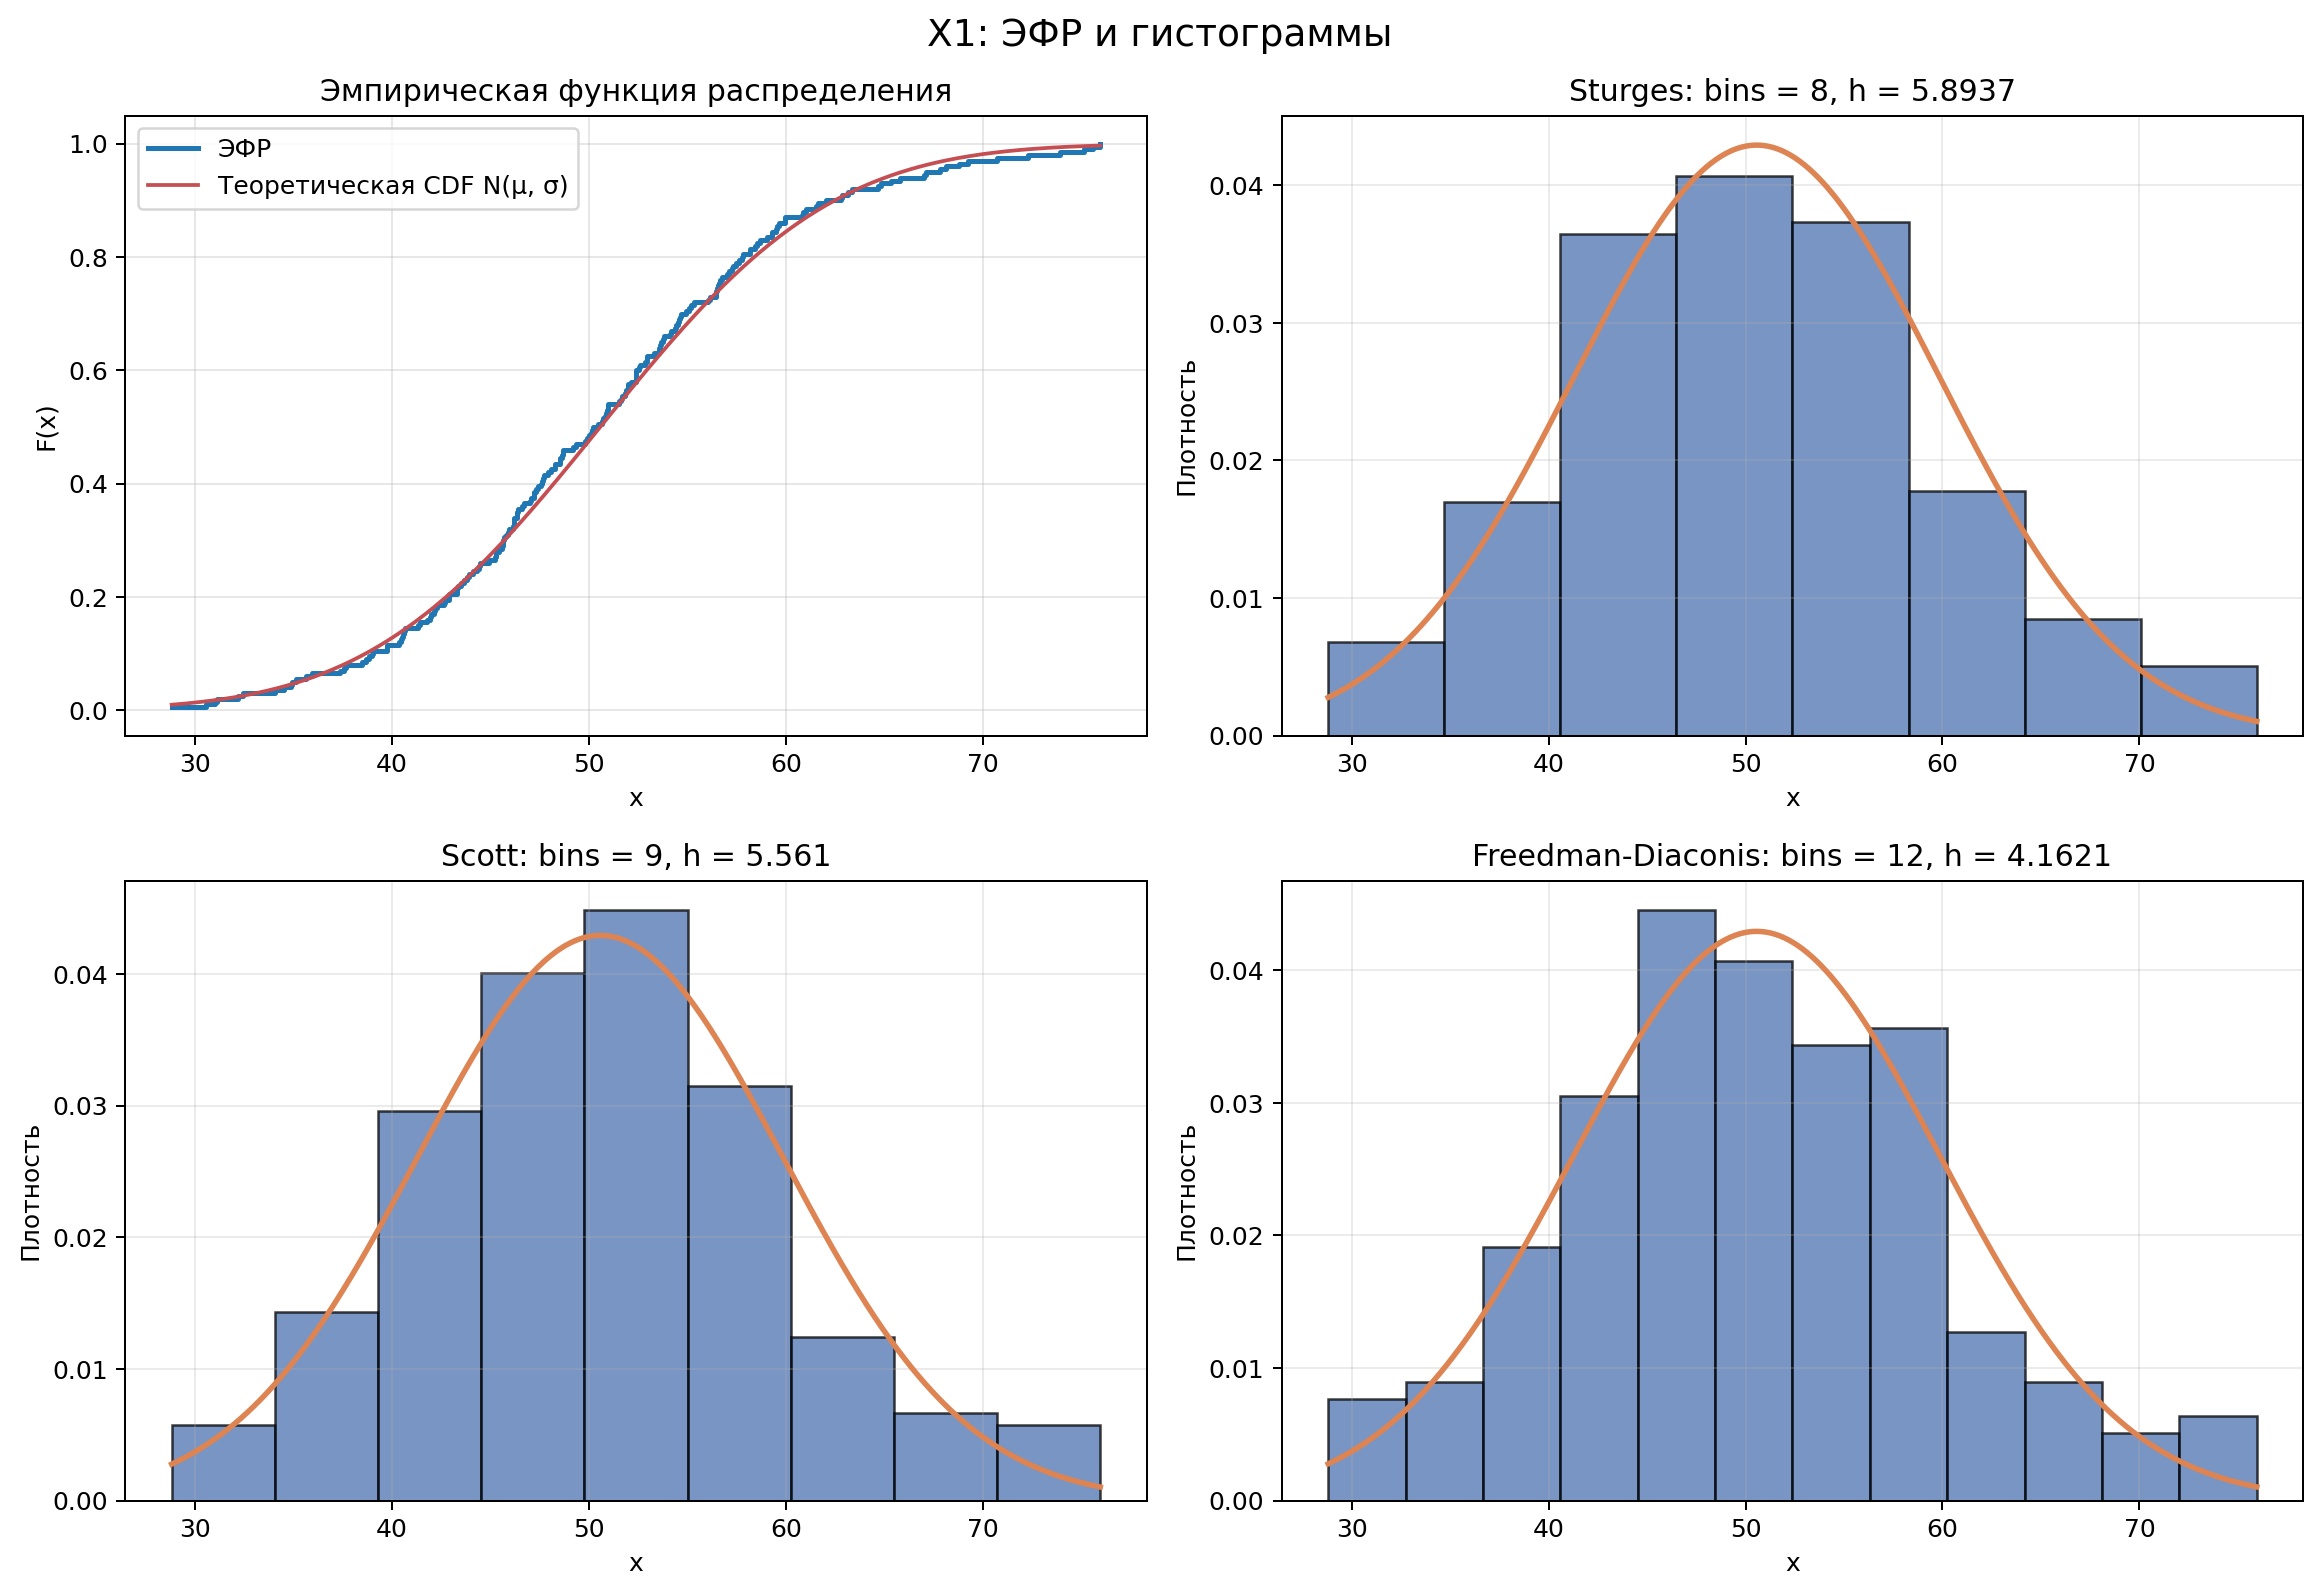
\includegraphics[width=\textwidth]{output/plots/X1_overview.png}
    \caption{Эмпирическая функция распределения и гистограммы для столбца X1}
\end{figure}

\subsection{Первичное описание выборки}

Фрагмент вариационного ряда приведён ниже; полный вариационный ряд вынесен в приложение и сохранён в \texttt{output/variation\_series/X1\_variation\_series.csv}.

\begin{center}
\begin{tabular}{rr}
\toprule
$i$ & $x_{(i)}$ \\
\midrule
1 & 28.81 \\
2 & 30.54 \\
3 & 31.03 \\
4 & 31.11 \\
5 & 32.17 \\
\dots & \dots \\
196 & 72.30 \\
197 & 73.92 \\
198 & 75.15 \\
199 & 75.60 \\
200 & 75.96 \\
\bottomrule
\end{tabular}
\end{center}

\subsubsection*{Числовые характеристики}

\begin{center}
\begin{tabular}{>{\raggedright\arraybackslash}p{0.55\textwidth}r}
\toprule
Показатель & Значение \\
\midrule
$n$ & 200 \\
$\min$ & 28.81 \\
$\max$ & 75.96 \\
Среднее $\bar{x}$ & 50.5689 \\
Смещённая дисперсия $S^2$ & 86.3364 \\
Несмещённая дисперсия $\hat{\sigma}^2$ & 86.7702 \\
$S$ & 9.2917 \\
$\hat{\sigma}$ & 9.3151 \\
Медиана & 50.3350 \\
$q_{0.10}$ & 39.0090 \\
$q_{0.25}$ & 44.3900 \\
$q_{0.75}$ & 56.5600 \\
$q_{0.90}$ & 62.0910 \\
Асимметрия & 0.2686 \\
\bottomrule
\end{tabular}
\end{center}

Распределение близко к симметричному: коэффициент асимметрии равен $0.2686$, среднее и медиана практически совпадают. Наблюдения лежат в диапазоне $[28.81; 75.96]$, выраженной естественной границы нет.

\subsection{Предположение о виде закона распределения}

По визуальной форме гистограммы и ЭФР лучше всего подходит нормальное распределение. Дополнительно использована KS-подобная метрика для трёх моделей: $N(\mu, \sigma)$ --- $0.0401$, $U(a,b)$ --- $0.2091$, $\mathrm{Exp}(\lambda,c)$ --- $0.2919$.

\subsection{Оценивание параметров: метод моментов и метод максимального правдоподобия}

\textbf{Метод моментов.}

Теоретические моменты:
\[
\mathbb{E}X = \mu, \qquad \mathbb{D}X = \sigma^2.
\]
Приравниваем их выборочным характеристикам:
\[
\mu = \bar{x} = 50.5689, \qquad \sigma^2 = S^2 = 86.3364.
\]
Отсюда
\[
\hat{\mu}_{MM} = 50.5689, \qquad \hat{\sigma}_{MM} = S = 9.2917.
\]

\textbf{Метод максимального правдоподобия.}

Логарифм правдоподобия:
\[
\ell(\mu,\sigma) = -n\ln\sigma - \frac{n}{2}\ln(2\pi) - \frac{1}{2\sigma^2}\sum_{i=1}^{n}(x_i-\mu)^2.
\]
Максимум достигается в точке
\[
\hat{\mu}_{MLE} = \bar{x} = 50.5689, \qquad \hat{\sigma}_{MLE}^2 = S^2 = 86.3364,
\]
то есть
\[
\hat{\sigma}_{MLE} = 9.2917.
\]

\begin{center}
\begin{tabular}{>{\raggedright\arraybackslash}p{0.35\textwidth}p{0.45\textwidth}}
\toprule
Метод & Оценки параметров \\
\midrule
Метод моментов & $\mu = 50.5689$, $\sigma = 9.2917$ \\
ММП & $\mu = 50.5689$, $\sigma = 9.2917$ \\
\bottomrule
\end{tabular}
\end{center}

Оценки метода моментов и ММП совпадают.

\subsection{Оценивание параметрической вероятности двумя способами}

Выбран порог
\[
x_0 = \bar{x} + \hat{\sigma} = 59.884.
\]
Эмпирическая оценка:
\[
\widehat{P}(X > x_0) = 0.14.
\]
Параметрическая оценка по методу моментов равна $0.158$, по ММП --- $0.158$.

\subsection{Оценка моментов по сгруппированной выборке}

\begin{center}
\begin{tabular}{lrr}
\toprule
Оценка & По исходной выборке & По сгруппированной выборке \\
\midrule
$\mathbb{E}X$ & 50.5689 & 50.5186 \\
$\mathbb{D}X$ & 86.7702 & 89.1293 \\
\bottomrule
\end{tabular}
\end{center}

\subsection{Доверительные интервалы}

Асимптотический 95\% доверительный интервал для $\mathbb{E}X$:
\[
(49.2779;\, 51.8599).
\]

Точный 95\% доверительный интервал для $\mu$:
\[
(49.2700;\, 51.8678).
\]

Точный 95\% доверительный интервал для $\sigma^2$:
\[
(71.9591;\, 106.7026).
\]

Интервал доверия 95\% означает, что при многократном повторении процедуры выборки и построения интервалов примерно 95\% построенных интервалов будут накрывать истинный параметр. Это не вероятность того, что уже после наблюдения данных параметр лежит в конкретном интервале.

\section{Столбец X2}

Модель: \textbf{$U(a,b)$}.

\begin{figure}[H]
    \centering
    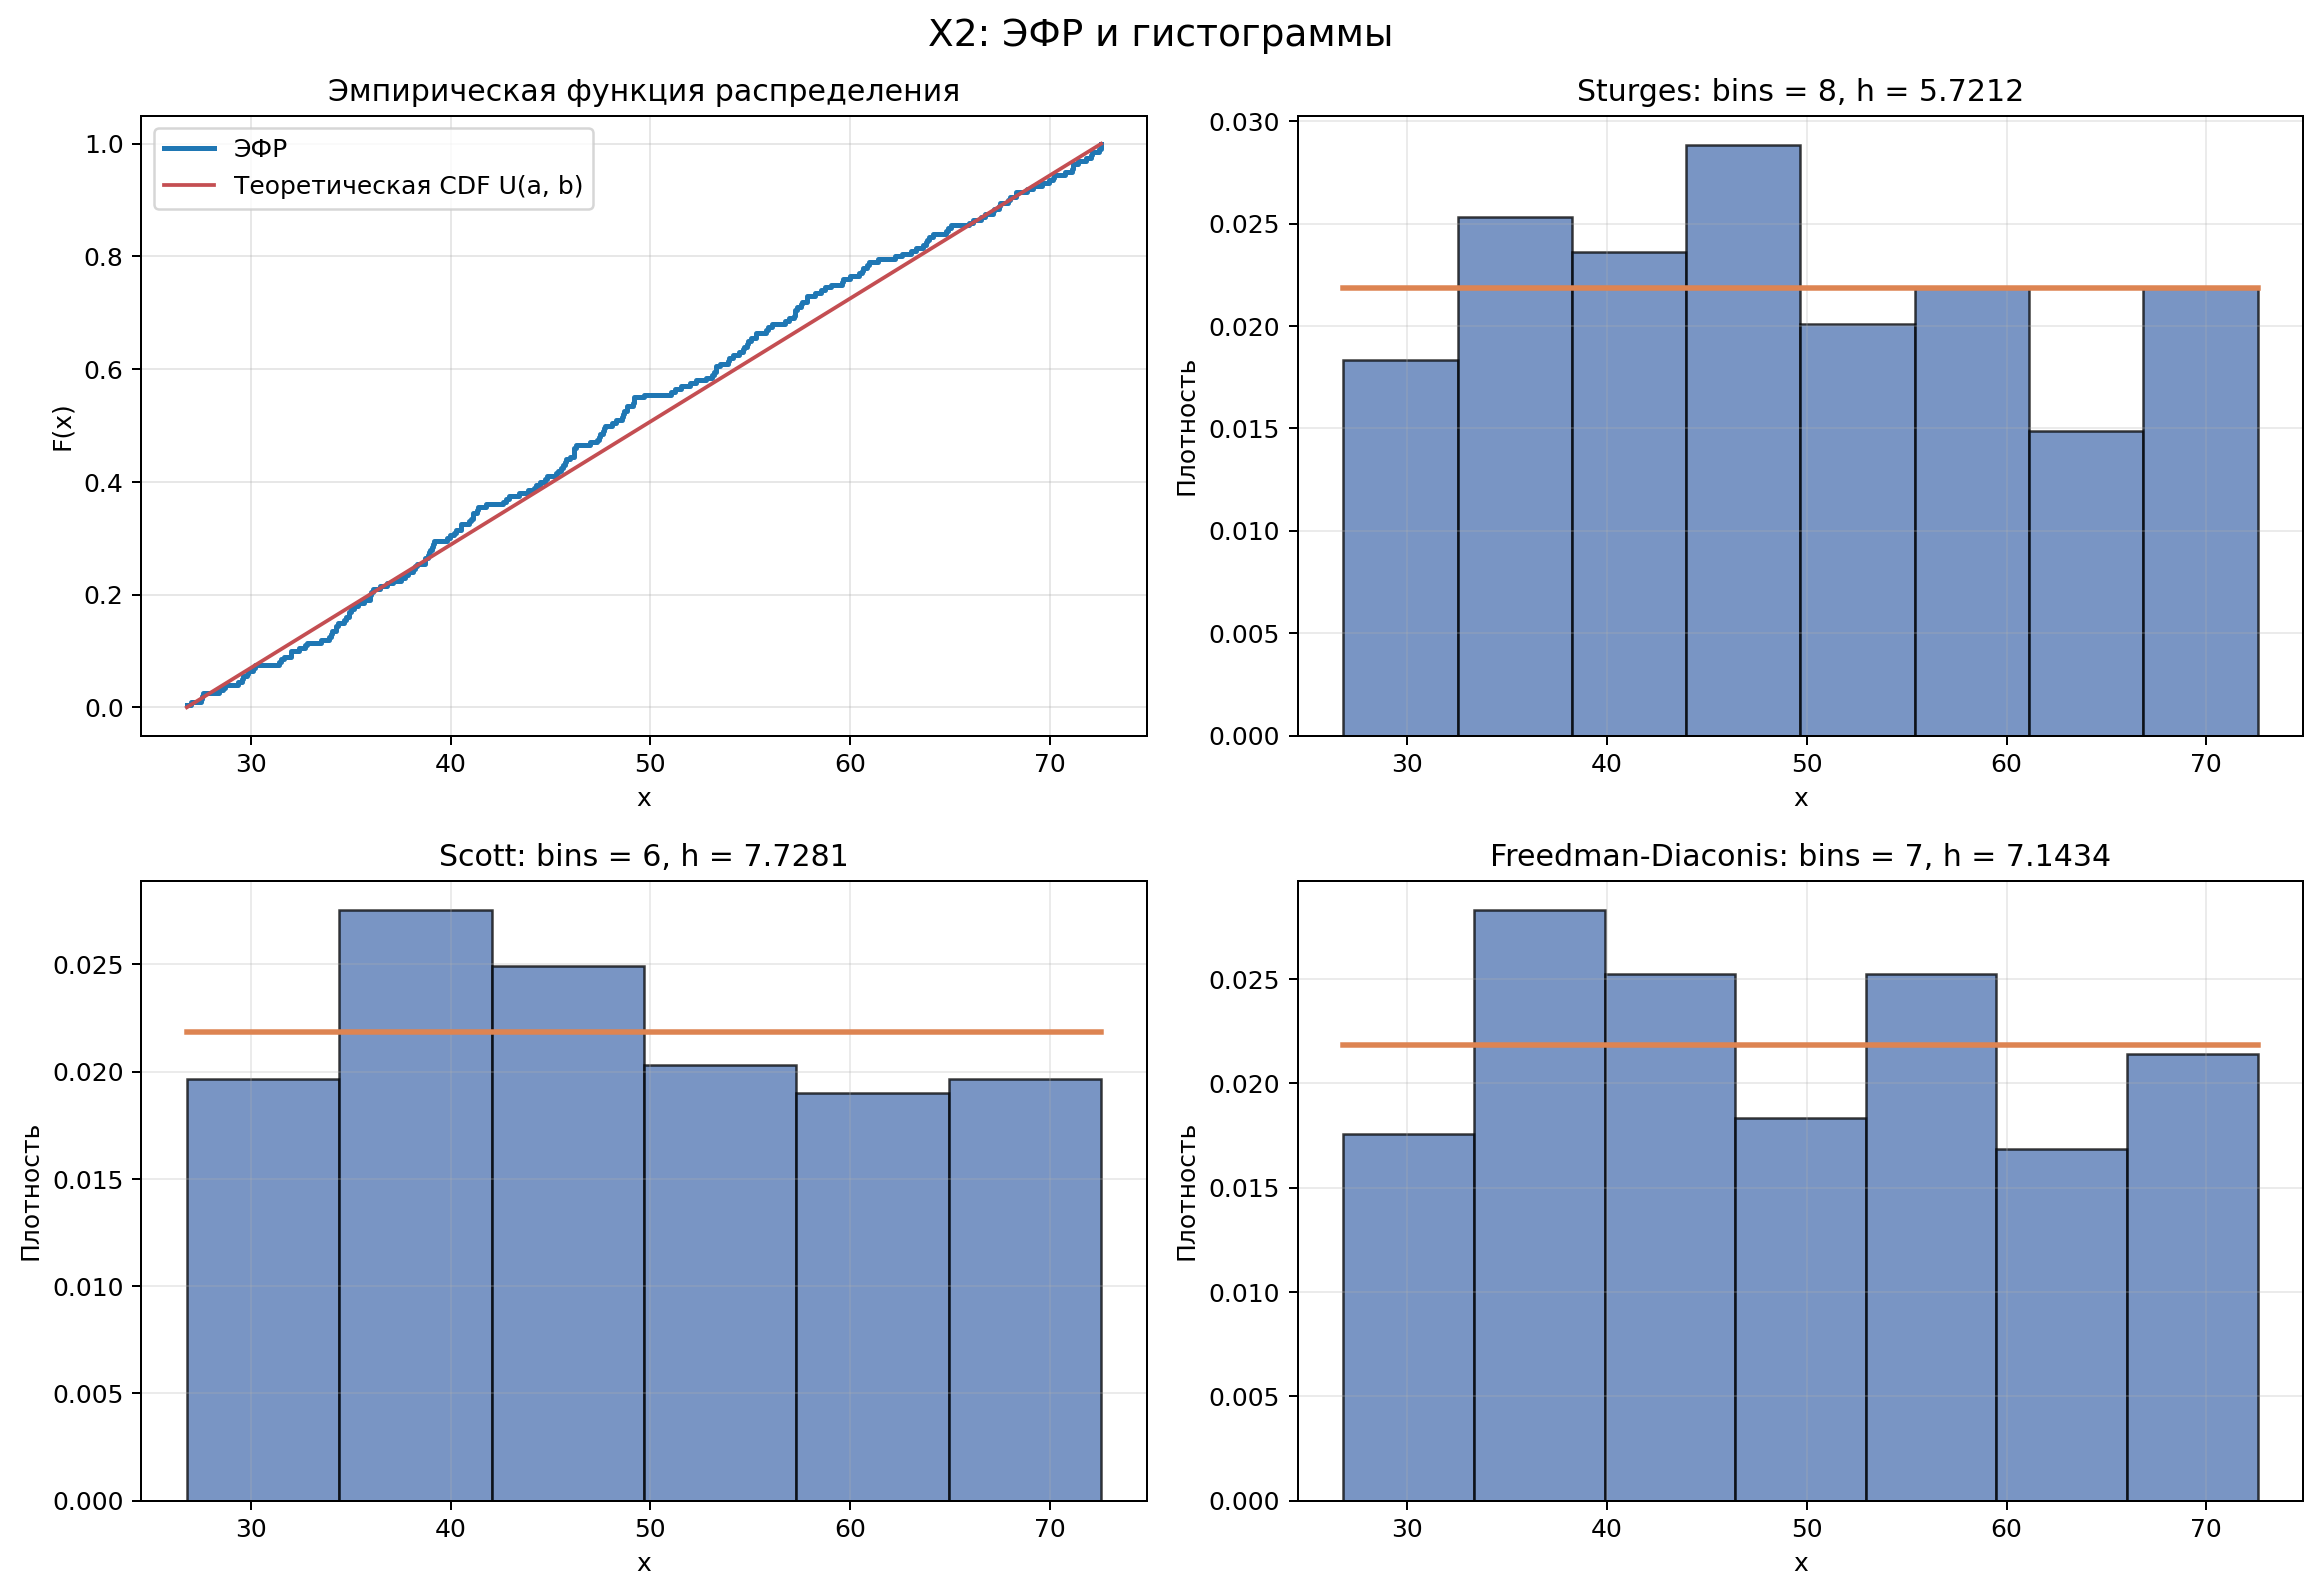
\includegraphics[width=\textwidth]{output/plots/X2_overview.png}
    \caption{Эмпирическая функция распределения и гистограммы для столбца X2}
\end{figure}

\subsection{Первичное описание выборки}

Фрагмент вариационного ряда:

\begin{center}
\begin{tabular}{rr}
\toprule
$i$ & $x_{(i)}$ \\
\midrule
1 & 26.80 \\
2 & 27.00 \\
3 & 27.53 \\
4 & 27.57 \\
5 & 27.62 \\
\dots & \dots \\
196 & 72.04 \\
197 & 72.11 \\
198 & 72.46 \\
199 & 72.54 \\
200 & 72.57 \\
\bottomrule
\end{tabular}
\end{center}

\subsubsection*{Числовые характеристики}

\begin{center}
\begin{tabular}{>{\raggedright\arraybackslash}p{0.55\textwidth}r}
\toprule
Показатель & Значение \\
\midrule
$n$ & 200 \\
$\min$ & 26.80 \\
$\max$ & 72.57 \\
Среднее $\bar{x}$ & 49.0995 \\
Смещённая дисперсия $S^2$ & 166.7376 \\
Несмещённая дисперсия $\hat{\sigma}^2$ & 167.5754 \\
$S$ & 12.9127 \\
$\hat{\sigma}$ & 12.9451 \\
Медиана & 47.9000 \\
$q_{0.10}$ & 32.3540 \\
$q_{0.25}$ & 38.2875 \\
$q_{0.75}$ & 59.1750 \\
$q_{0.90}$ & 67.9360 \\
Асимметрия & 0.1442 \\
\bottomrule
\end{tabular}
\end{center}

Данные почти равномерно заполняют интервал $[26.8; 72.57]$. Асимметрия мала, среднее и медиана близки, выраженного хвоста нет.

\subsection{Предположение о виде закона распределения}

Лучше всего подходит равномерное распределение. KS-подобная метрика: $U(a,b)$ --- $0.0606$, $N(\mu,\sigma)$ --- $0.0795$, $\mathrm{Exp}(\lambda,c)$ --- $0.1535$.

\subsection{Оценивание параметров: метод моментов и метод максимального правдоподобия}

\textbf{Метод моментов.}
\[
\mathbb{E}X = \frac{a+b}{2}, \qquad \mathbb{D}X = \frac{(b-a)^2}{12}.
\]
Система метода моментов:
\[
\frac{a+b}{2} = \bar{x} = 49.0995, \qquad \frac{(b-a)^2}{12} = S^2 = 166.7376.
\]
Отсюда
\[
\hat{a}_{MM} = 26.7341, \qquad \hat{b}_{MM} = 71.4649.
\]

\textbf{Метод максимального правдоподобия.}

Функция правдоподобия:
\[
L(a,b) = (b-a)^{-n}\, I\{a \le x_{(1)}, x_{(n)} \le b\}.
\]
Тогда
\[
\ell(a,b) = -n \ln(b-a)
\]
при выполнении ограничений на носитель. Чтобы максимизировать $\ell(a,b)$, нужно минимизировать длину интервала, содержащего всю выборку. Поэтому
\[
\hat{a}_{MLE} = x_{(1)} = 26.80, \qquad \hat{b}_{MLE} = x_{(n)} = 72.57.
\]

\begin{center}
\begin{tabular}{>{\raggedright\arraybackslash}p{0.35\textwidth}p{0.45\textwidth}}
\toprule
Метод & Оценки параметров \\
\midrule
Метод моментов & $a = 26.7341$, $b = 71.4649$ \\
ММП & $a = 26.8000$, $b = 72.5700$ \\
\bottomrule
\end{tabular}
\end{center}

\subsection{Оценивание параметрической вероятности двумя способами}

Порог:
\[
x_0 = \bar{x} + \hat{\sigma} = 62.0446.
\]
Эмпирическая оценка вероятности $P(X > x_0)$ равна $0.205$. Параметрическая оценка по методу моментов равна $0.2106$, по ММП --- $0.23$.

\subsection{Оценка моментов по сгруппированной выборке}

\begin{center}
\begin{tabular}{lrr}
\toprule
Оценка & По исходной выборке & По сгруппированной выборке \\
\midrule
$\mathbb{E}X$ & 49.0995 & 49.1946 \\
$\mathbb{D}X$ & 167.5754 & 163.2506 \\
\bottomrule
\end{tabular}
\end{center}

\subsection{Доверительные интервалы}

Асимптотический 95\% доверительный интервал для $\mathbb{E}X$:
\[
(47.3054;\, 50.8936).
\]

\section{Столбец X3}

Модель: \textbf{$\mathrm{Exp}(\lambda,c)$}.

\begin{figure}[H]
    \centering
    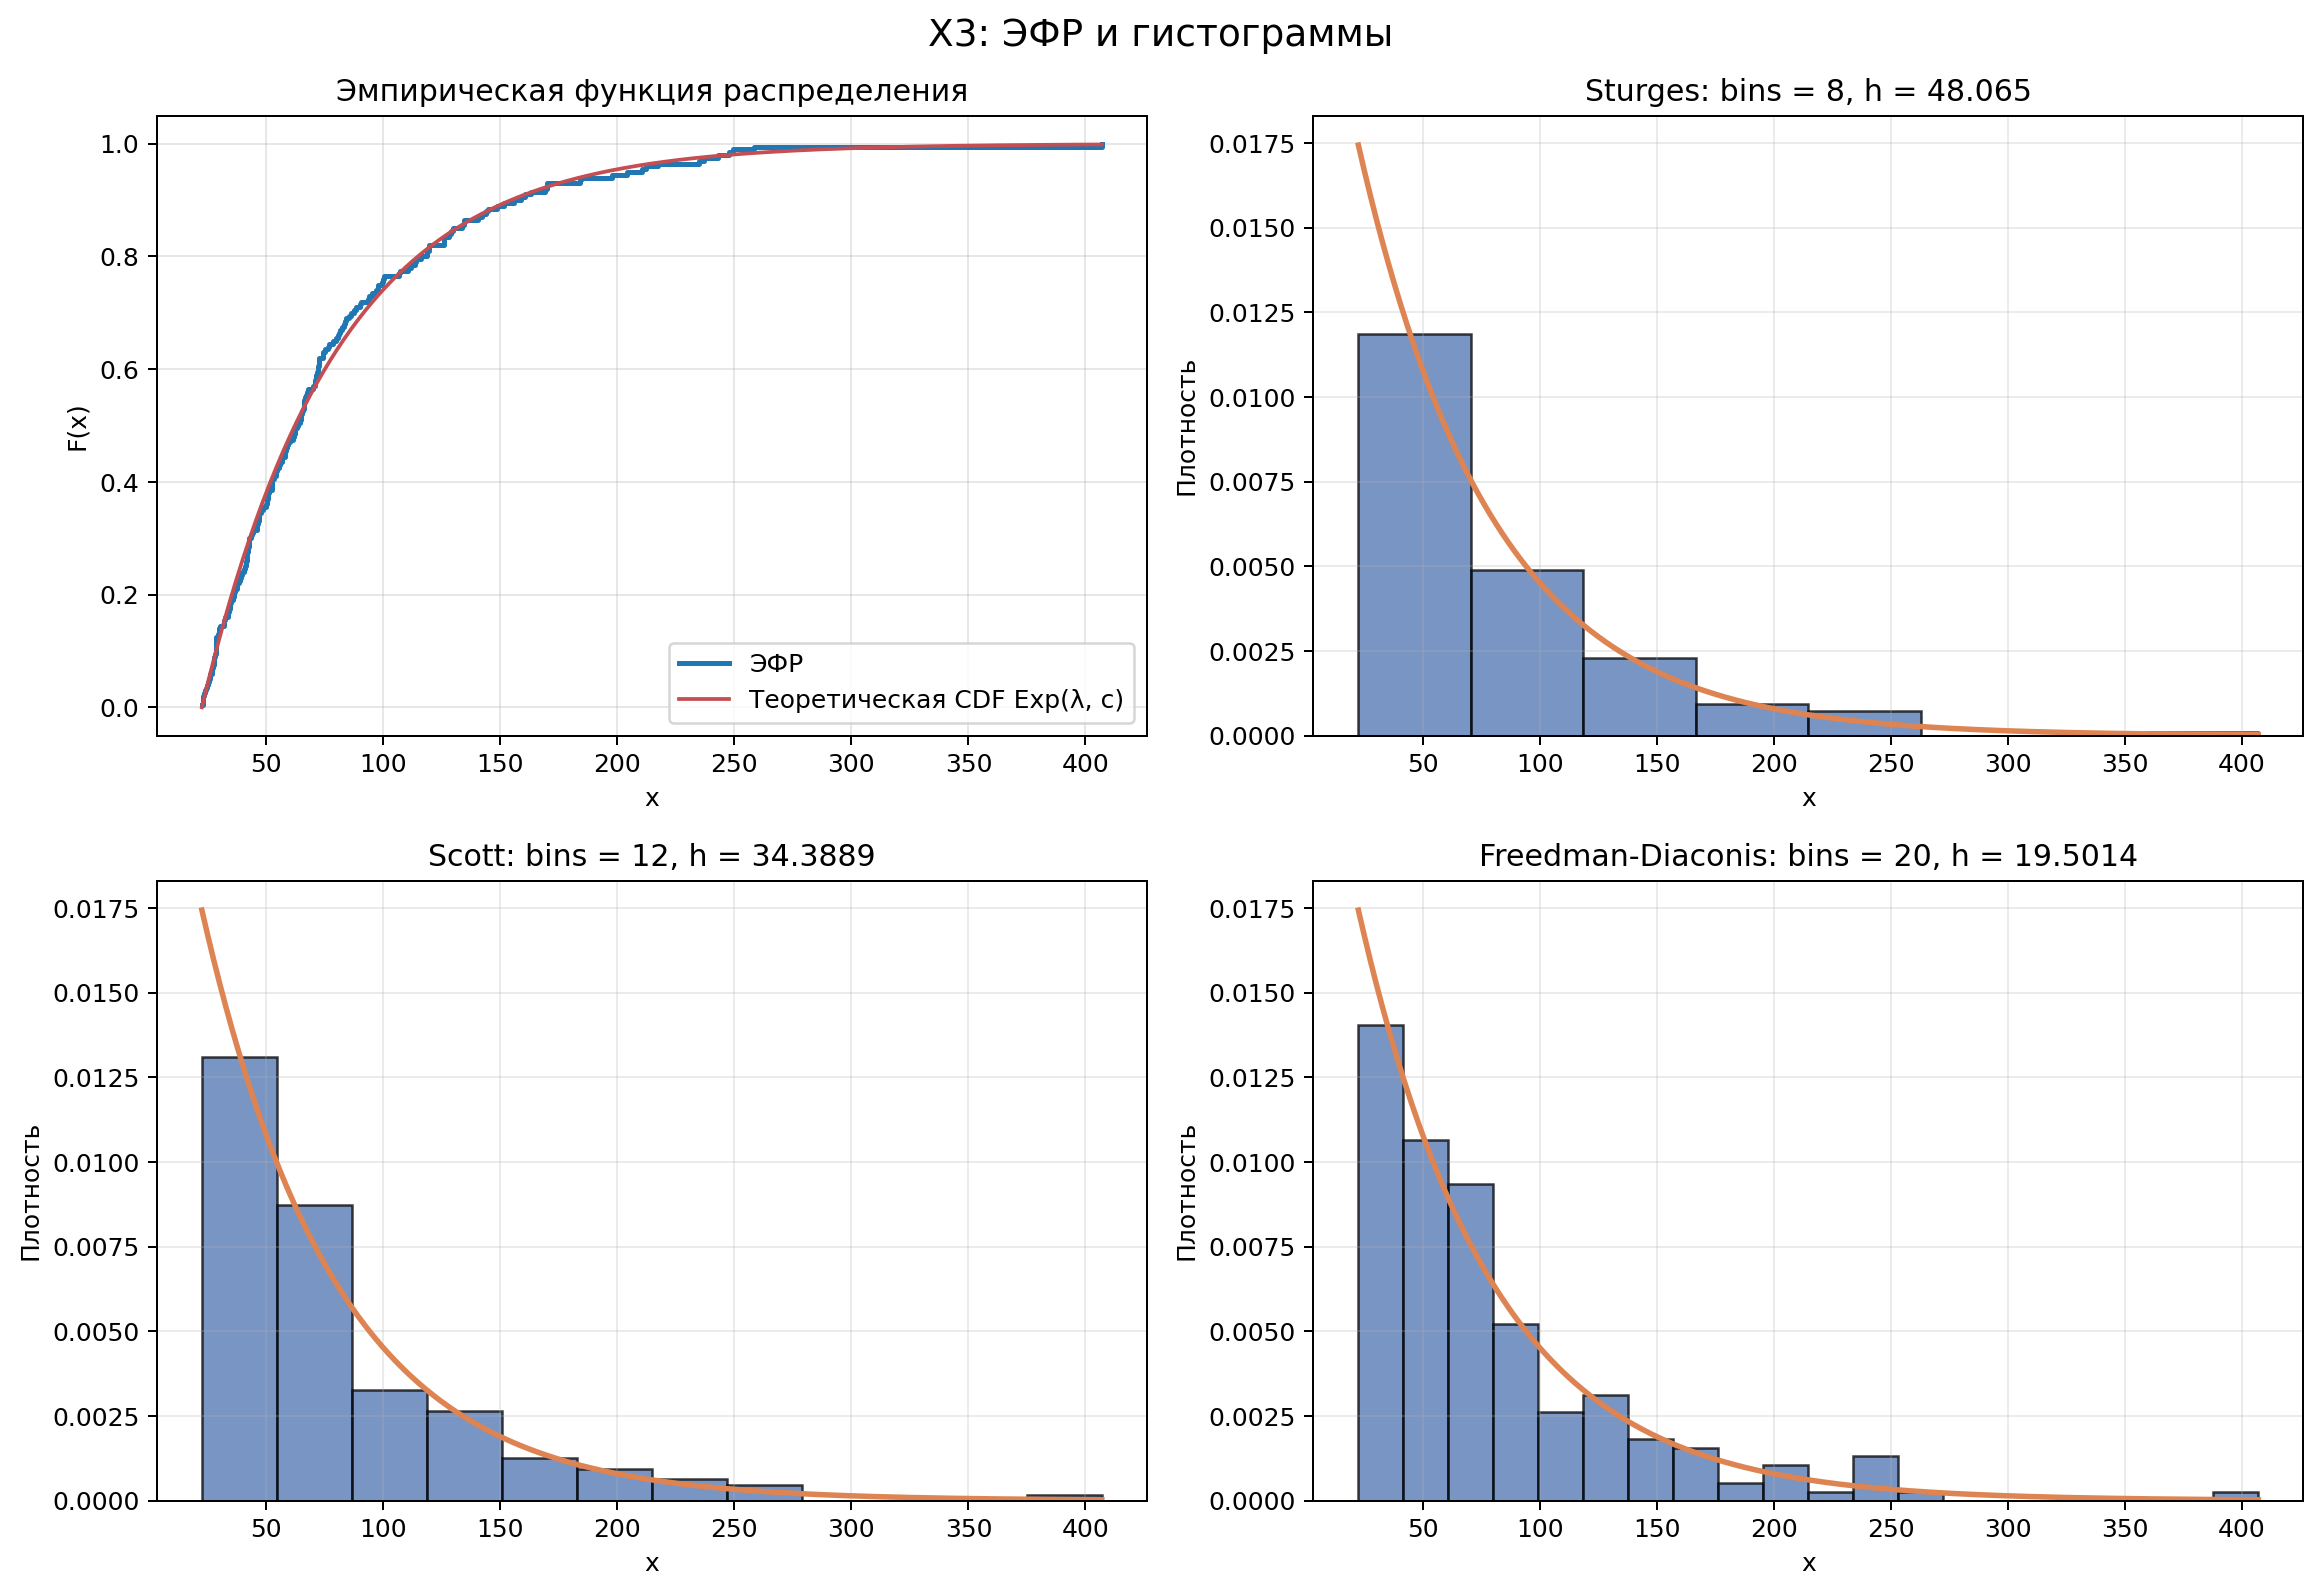
\includegraphics[width=\textwidth]{output/plots/X3_overview.png}
    \caption{Эмпирическая функция распределения и гистограммы для столбца X3}
\end{figure}

\subsection{Первичное описание выборки}

Фрагмент вариационного ряда:

\begin{center}
\begin{tabular}{rr}
\toprule
$i$ & $x_{(i)}$ \\
\midrule
1 & 22.47 \\
2 & 22.76 \\
3 & 22.89 \\
4 & 22.98 \\
5 & 23.53 \\
\dots & \dots \\
196 & 242.97 \\
197 & 247.71 \\
198 & 249.20 \\
199 & 258.37 \\
200 & 406.99 \\
\bottomrule
\end{tabular}
\end{center}

\subsubsection*{Числовые характеристики}

\begin{center}
\begin{tabular}{>{\raggedright\arraybackslash}p{0.55\textwidth}r}
\toprule
Показатель & Значение \\
\midrule
$n$ & 200 \\
$\min$ & 22.47 \\
$\max$ & 406.99 \\
Среднее $\bar{x}$ & 79.8089 \\
Смещённая дисперсия $S^2$ & 3301.5753 \\
Несмещённая дисперсия $\hat{\sigma}^2$ & 3318.1661 \\
$S$ & 57.4593 \\
$\hat{\sigma}$ & 57.6035 \\
Медиана & 63.3500 \\
$q_{0.10}$ & 28.3460 \\
$q_{0.25}$ & 41.1600 \\
$q_{0.75}$ & 98.1825 \\
$q_{0.90}$ & 156.2110 \\
Асимметрия & 1.9827 \\
\bottomrule
\end{tabular}
\end{center}

Выборка имеет сильную правостороннюю асимметрию, минимум задаёт естественную левую границу, а правый хвост заметно растянут. Среднее существенно больше медианы.

\subsection{Предположение о виде закона распределения}

Лучше всего подходит экспоненциальное распределение со сдвигом. KS-подобная метрика: $\mathrm{Exp}(\lambda,c)$ --- $0.0364$, $N(\mu,\sigma)$ --- $0.1692$, $U(a,b)$ --- $0.5732$.

\subsection{Оценивание параметров: метод моментов и метод максимального правдоподобия}

\textbf{Метод моментов.}
\[
\mathbb{E}X = c + \frac{1}{\lambda}, \qquad \mathbb{D}X = \frac{1}{\lambda^2}.
\]
Система:
\[
c + \frac{1}{\lambda} = \bar{x} = 79.8089, \qquad \frac{1}{\lambda^2} = S^2 = 3301.5753.
\]
Отсюда
\[
\hat{\lambda}_{MM} = 0.0174, \qquad \hat{c}_{MM} = 22.3496.
\]

\textbf{Метод максимального правдоподобия.}

\[
L(\lambda, c) = \lambda^n \exp\left(-\lambda \sum_{i=1}^{n}(x_i-c)\right) I\{c \le x_{(1)}\}.
\]
\[
\ell(\lambda,c) = n\ln\lambda - \lambda \sum_{i=1}^{n}(x_i-c), \qquad c \le x_{(1)}.
\]
Максимум достигается при
\[
\hat{c}_{MLE} = x_{(1)} = 22.47, \qquad \hat{\lambda}_{MLE} = \frac{1}{\bar{x} - \hat{c}} = 0.0174.
\]

\begin{center}
\begin{tabular}{>{\raggedright\arraybackslash}p{0.35\textwidth}p{0.45\textwidth}}
\toprule
Метод & Оценки параметров \\
\midrule
Метод моментов & $\lambda = 0.0174$, $c = 22.3496$ \\
ММП & $\lambda = 0.0174$, $c = 22.4700$ \\
\bottomrule
\end{tabular}
\end{center}

\subsection{Оценивание параметрической вероятности двумя способами}

Порог:
\[
x_0 = \bar{x} + \hat{\sigma} = 137.4124.
\]
Эмпирическая оценка $P(X > x_0)$ равна $0.135$. Параметрическая оценка по методу моментов равна $0.1350$, по ММП --- $0.1347$.

\subsection{Оценка моментов по сгруппированной выборке}

\begin{center}
\begin{tabular}{lrr}
\toprule
Оценка & По исходной выборке & По сгруппированной выборке \\
\midrule
$\mathbb{E}X$ & 79.8089 & 80.6286 \\
$\mathbb{D}X$ & 3318.1661 & 3265.2226 \\
\bottomrule
\end{tabular}
\end{center}

\subsection{Доверительные интервалы}

Асимптотический 95\% доверительный интервал для $\mathbb{E}X$:
\[
(71.8256;\, 87.7922).
\]

\section{Столбец X4}

\begin{figure}[H]
    \centering
    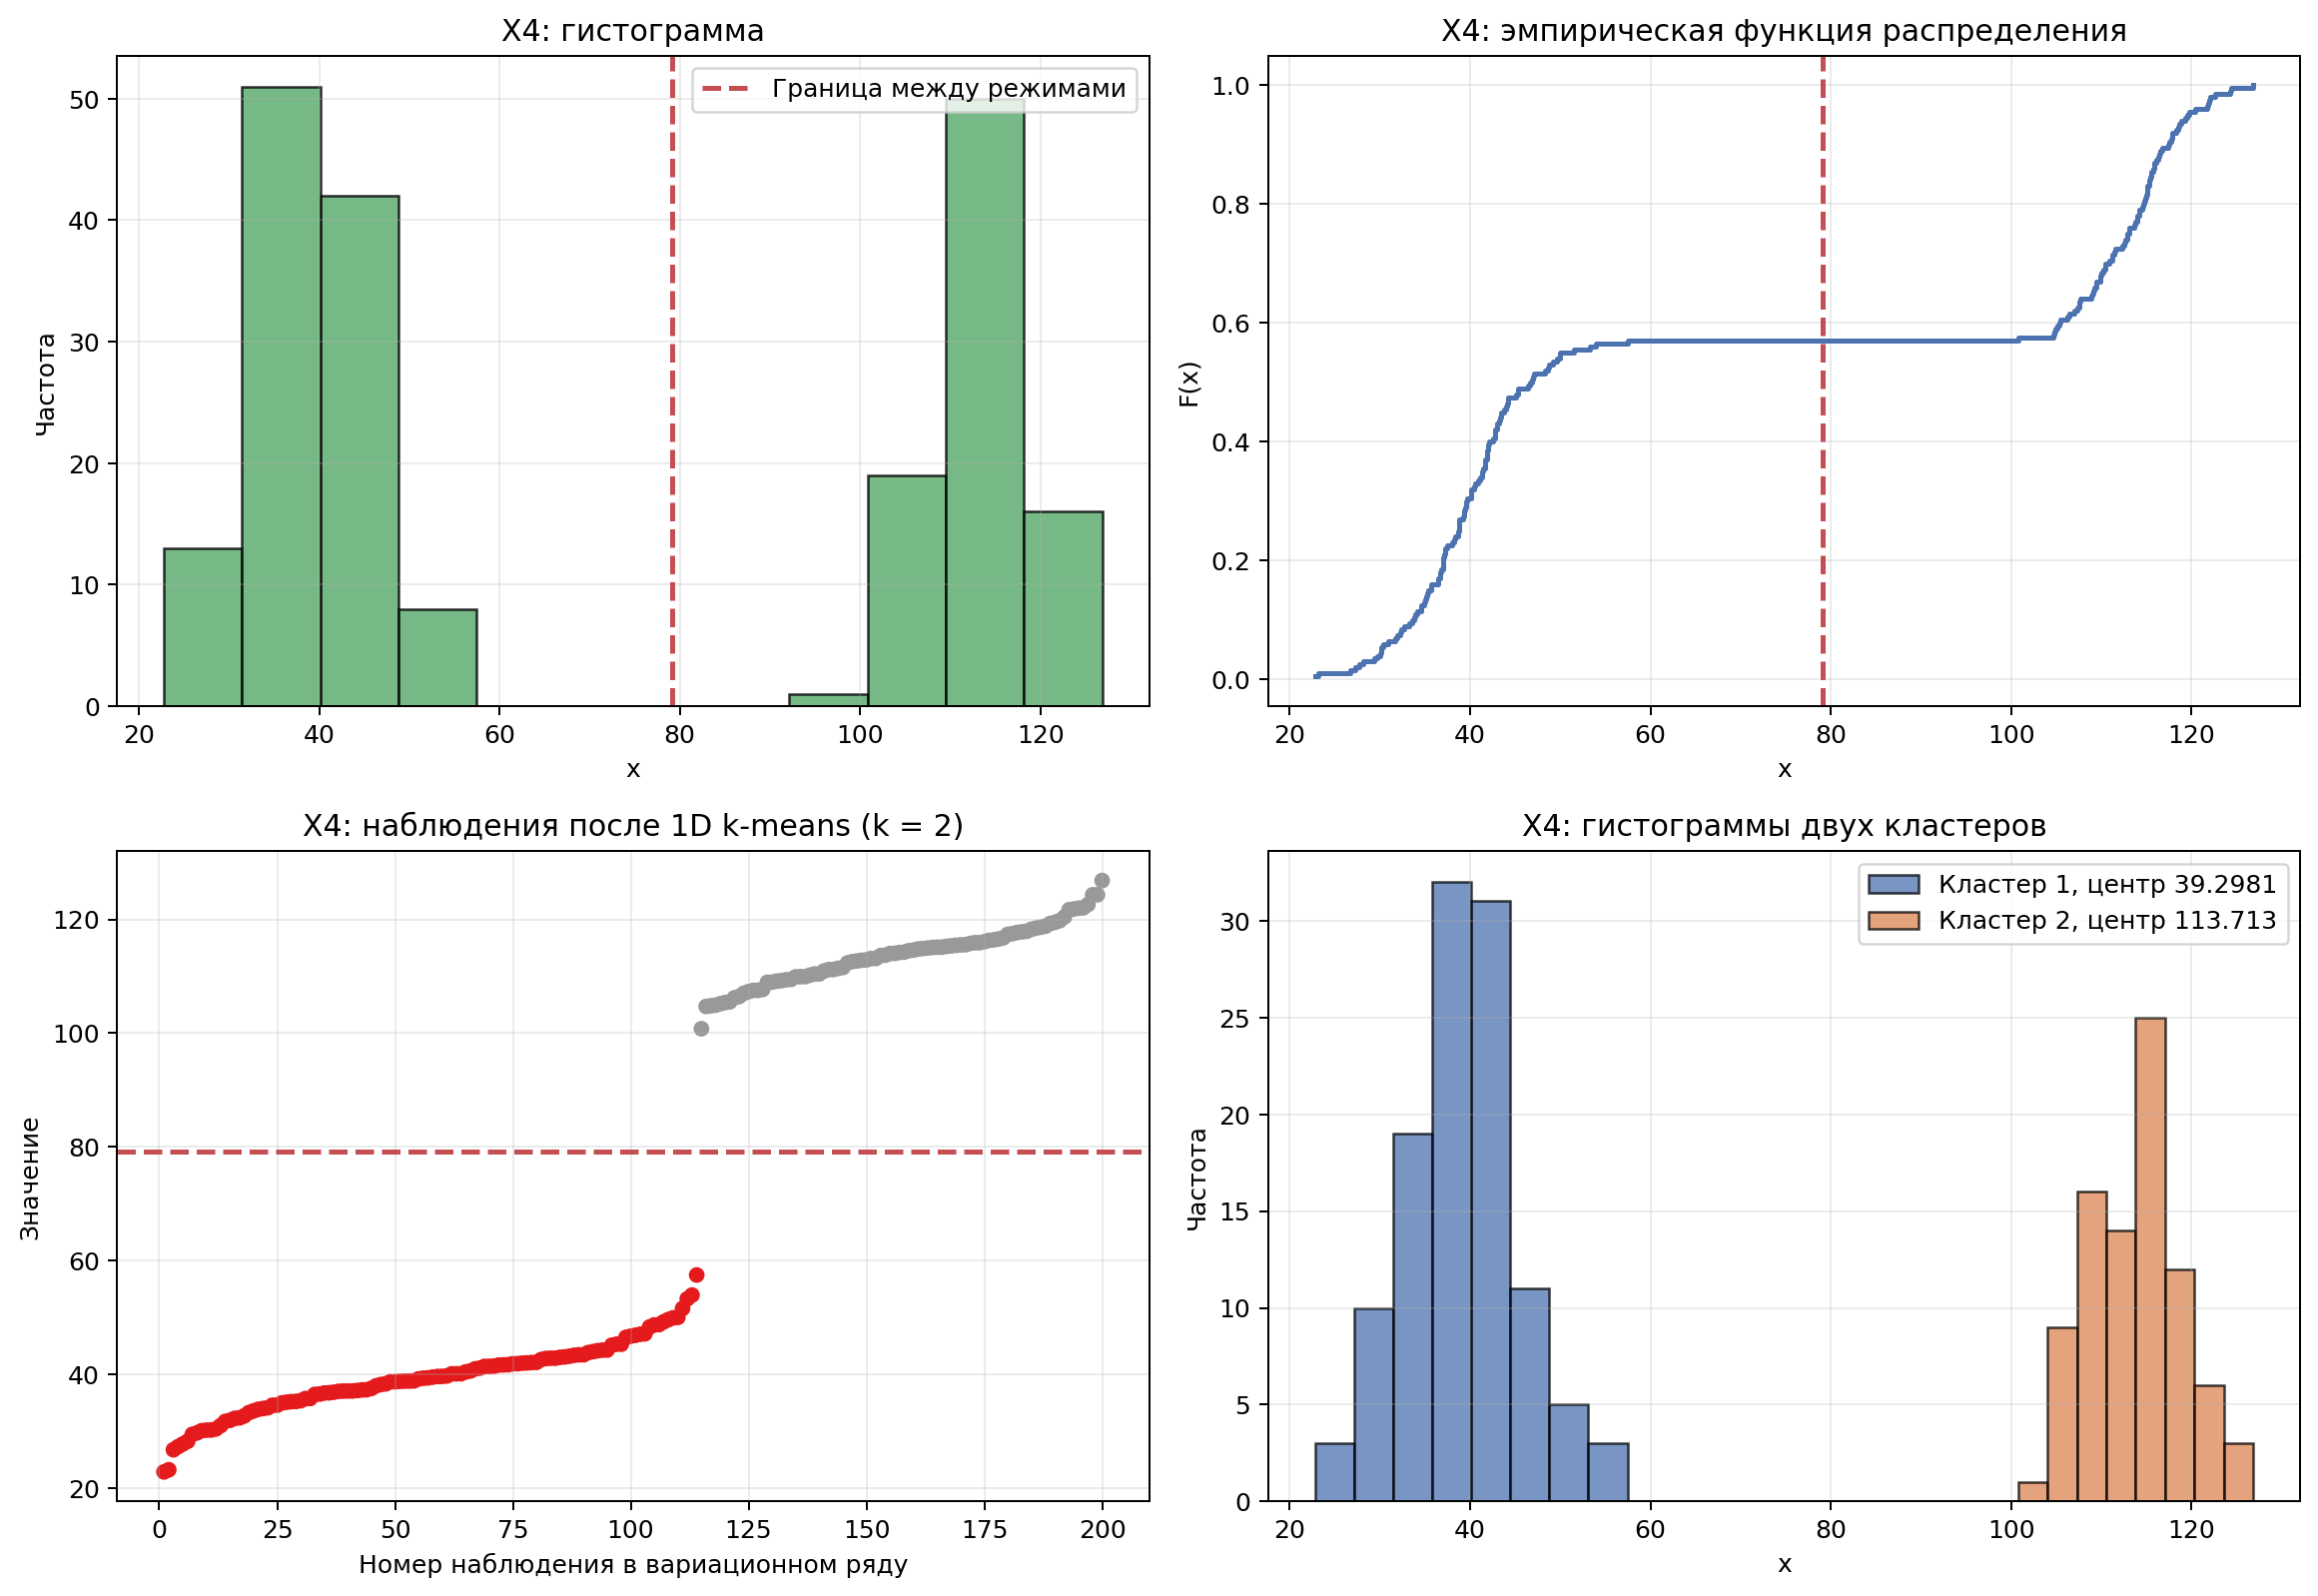
\includegraphics[width=\textwidth]{output/plots/X4_overview.png}
    \caption{Гистограмма, эмпирическая функция распределения и кластеризация для столбца X4}
\end{figure}

\subsection{Первичное описание выборки}

\begin{center}
\begin{tabular}{>{\raggedright\arraybackslash}p{0.55\textwidth}r}
\toprule
Показатель & Значение \\
\midrule
$n$ & 200 \\
$\min$ & 22.80 \\
$\max$ & 126.84 \\
Среднее $\bar{x}$ & 71.2965 \\
Несмещённая дисперсия $\hat{\sigma}^2$ & 1398.9431 \\
$\hat{\sigma}$ & 37.4024 \\
Медиана & 46.7600 \\
$q_{0.25}$ & 38.7125 \\
$q_{0.75}$ & 112.9400 \\
Асимметрия & 0.2577 \\
\bottomrule
\end{tabular}
\end{center}

На рисунке для $X_4$ показаны и гистограмма, и эмпирическая функция распределения. ЭФР демонстрирует резкий переход между двумя группами значений. Между $57.44$ и $100.77$ наблюдается большой разрыв, а медиана заметно ниже среднего, что является признаком смеси двух режимов.

\subsection{Бонус: разбиение на 2 кластера}

\begin{center}
\begin{tabular}{rrrrrrr}
\toprule
Кластер & $n$ & $\min$ & $\max$ & Среднее & Медиана & $\hat{\sigma}$ \\
\midrule
1 & 114 & 22.80 & 57.44 & 39.2981 & 39.41 & 6.4048 \\
2 & 86 & 100.77 & 126.84 & 113.7130 & 114.21 & 5.2039 \\
\bottomrule
\end{tabular}
\end{center}

Алгоритм 1D k-means с $k = 2$ разделил выборку на два устойчивых кластера с центрами $39.2981$ и $113.7130$. Общее среднее плохо описывает такую смесь, потому что ни один из режимов не сосредоточен около $\bar{x} = 71.2965$.

\section{Итоговый вывод}

Для $X_1$ выбрана модель $N(\mu,\sigma)$: выборка почти симметрична, оценки параметров по методу моментов и ММП совпадают, а доверительные интервалы для среднего достаточно узкие.

Для $X_2$ выбрана модель $U(a,b)$: данные достаточно равномерно заполняют интервал, а различие между методом моментов и ММП связано с использованием крайних наблюдений в ММП.

Для $X_3$ выбрана модель $\mathrm{Exp}(\lambda,c)$: наблюдается выраженная правосторонняя асимметрия и естественная левая граница. Эмпирические и параметрические оценки вероятности события $P(X > x_0)$ практически совпадают, что подтверждает выбранную модель.

Столбец $X_4$ по форме похож на смесь двух подвыборок. Поэтому его корректнее описывать не одним средним, а отдельно по двум режимам.

\section{Приложение}

Полные вариационные ряды сохранены в папке \texttt{output/variation\_series} и могут быть приложены к отчёту отдельно.

\end{document}
